\section{Создание программного средства}
\label{sec:creation}

\subsection{Выбор языка программирования}
Исходя из опыта работы разработчика и поставленной задачи целесообразное всего использовать язык \csharp{} платформы \dotnet{}.


\subsection{Реализация архитектуры}
В разделе \ref{sec:arch_arch} была рассмотренна архитектура програмного средства и было определенно что разные части приложения буду иметь следующую архитектуру:
\begin{itemize}
	\item клиен-сервер
	\item каналы и фильтры
	\item микроядерная архитектура
\end{itemize}
Рассмотрим технические средства помогающие реализовать приведенный функционал.

\subsubsection{}
Клиент-сервер

Для реализации програмного средства как клиент-сервер можно использовать следующие фреймворки:
\begin{itemize}
	\item ASP.NET MVC
	\item NancyFx
\end{itemize}
Оба фреймовка предоставляют отличный возможности для создания веб приложений, но я выбрал именно nancyFx из-за его простого развертывания. Для запуска NancyFx можно использовать IIS, WCF и OWIN.


\subsubsection{}
Каналы и фильтры

Для реализации каналов и фильтров пока нету готовых фреймворков, есть лишь пример реализации архитектурного шаблона от Microsoft для платформы c использованием языка \csharp{} \cite{pipes_and_filters_pattern}, на рисунке \ref{fig:creation:pipes_and_filters_microsoft} можно увидеть схему работы шаблона.

\begin{figure}[ht] 
    \centering
    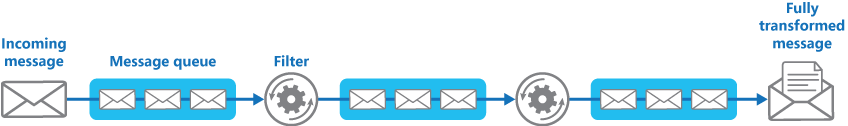
\includegraphics[scale=0.5]{pipes_and_filters_microsoft.png}  
    \caption{Схема реализации шаблона <<Каналы и фильтры>> от Microsoft}
    \label{fig:creation:pipes_and_filters_microsoft}
\end{figure}

Описанная реализация фокусируется на возможности распределенных вычислений которая в контексте обработки изображений бесполезно, поскольку производительность полученная от распределения фильтров на различные машины будет нивелированна временем затраченным передачу обрабатываемого изображения по сети. Главная цель при при использовании шаблона <<Каналы и фильтры>> в данном программном средстве это улучшение качества кода с точки зрения читаемости и модифицируемости. Декомпозиция кода на отдельные фильтры обработчики помогает упростить тестирование и реализацию отдельных модулей а правильная реализация каналов поможет в понимании связи фильтров и того что в целом происходит при обработке изображения. 

Прежде чем приступить к рассмотрению иходного кода требуется определить вспомогательные классы. 
В листинге \ref{lst:result_class} можно найти определение класса Result. Данный класс предназначен для упрощения обработки ошибок: все методы которые могут завершится неудачей должны возвращать класс Result не создавая при этом исключительных ситуаций. Использование описанной техники вместо исключительных ситуаций делает код понятнее потому как он исполняется последовательно как этого требует структурное программирование \cite{structured_programming}. Так же в программном средстве используется техника помогающая бороться с ошибками связанными с null значением. Это очень большая проблема для программистов! Техника состоит из 2 частей, первая это библиотека NullGuard \cite{null_guard}, которая встраивается в процесс компиляции и в начало каждого метода добавляет код проверяющий все входящие параметра на null значения, и в конец метода код проверяющий выходящее значение на null. Это запретит разработчику использовать null значения. Но для тех ситуаций где действительно значение может быть а может и не быть введем класс Maybe, код которого представлен на листинге \ref{lst:maybe}. Приведенный выше подход помогает четко разделить в коде значения которые могут принимать значения null а какие нет.

Рассмотрим реализацию архитектурного шаблона <<Каналы и фильтры>>. В листинге \ref{lst:ifilter} можно увидет определение интерфейса для фильтра. 
Интерфейс фильтр определяет сущность производящую определенную операцию над входящими данными и возвращающую результат либо ошибку. На изображении \ref{fig:creation:filters_uml} представленна UML диаграмма классов фильтров используемых в проекте.
\begin{figure}[ht] 
    \centering
    \includegraphics[width=\textwidth]{filters_uml.png}  
    \caption{UML диаграмма фильтров}
    \label{fig:creation:filters_uml}
\end{figure}

Перед рассмотрением каналов следует рассмотреть ещё один полезный при разработке прием это <<Dependency injection>> что означает на русском звучит как внедрение зависимостей, это процесс предоставления внешней зависимости программному модулю. Идея заключается в том что каждый модуль описывает свои зависимости, и выделяется отдельный модуль занимающийся предоставлением зависимостей. В \csharp{} хорошей практикой считается описывать зависимости именно в конструкторе класса. На внешний модуль занимающийся подстановкой возложенна задача управления жизненным циклом объектов а также их созданем, этот модуль называют <<IoC>>. В \dotnet{} существует масса реализаций, я же в своем проекте использую реализацию от Microsoft называемую Unity потому как при всей гибкости настроек и удобства использования, это реализация показал отличные результаты в плане производительности \cite{ioc_perfomance}.

И так при создании канала были следующие задачи:
\begin{itemize}
  \item обеспечение связи между фильтрами, т.е. передача данных между фильтрами;
  \item связи могут быть нелинейными;
  \item связи могу быть один ко многим и много к одному;
  \item при создании фильтров использовать технику <<Dependency injection>>;
  \item должна быть проверка совместимости типов фильтров на этапе компиляции;
\end{itemize}

Под нелинейными связями подразумевались связи при которых данные идут в обход некоторых фильтров попадая к следующим. Пример нелинейного соединения данных можно увидеть на рисунке \ref{fig:creation:unlinear_filter_connection}, тут данные из процесса 1 идет в обход процесса 2 и 3 к процессу 4.
\begin{figure}[ht] 
    \centering
    \includegraphics[width=0.95\textwidth]{unlinear_filter_connection.png}  
    \caption{Диаграмма потока данных при нелинейных связях фильтрах}
    \label{fig:creation:unlinear_filter_connection}
\end{figure}

На рисунке \ref{fig:creation:filters-one-to-many} изображен пример связи между фильтрами один ко многим, на диаграмме процесс 1 создает множество потоков данных, кажный из которых проходит другие процессы, затем процесс $n+1$ принимает множество потоков данных.
\begin{figure}[ht] 
    \centering
    \includegraphics[scale=0.6]{filters-one-to-many.png}  
    \caption{Диаграмма потока данных при связях фильтров один ко многим}
    \label{fig:creation:filters-one-to-many}
\end{figure}

Использование техники <<Dependency injection>> означает то, что каждый фильтр должен иметь возможность определить свои зависимости в конструкторе, при этом не вызывая ошибок компиляции после добавления новой зависимости.

Проверка совместимости типов фильтров на этапе компиляции означает то, что в случае совмещения выхода фильтра $A$ и входа фильтра $B$ код будет компилироваться только в том случае, если выходным значением фильтра $A$ будет тип $a$ а входным значением фильтра $B$ будет тип $b$ такие что $a \geq b$.

При реализации каналов хорошо подойдет прием программирования <<Fluent interface>> - способ реализации объектно-ориентированного API, нацеленный на повышение читабельности исходного кода программы.

В листинге \ref{lst:pipe} можно увидеть реализацию описанных выше функций.

Для реализации связей между фильтрами многие ко многим была использованна возможностью языка \csharp{} <<Метод расширение>>. Это возможность написать статический метод за пределами типа $A$ и принимающий первым параметром объект типа $A$, при чем вызов этого метода будет выглядеть как вызов метода у типа $A$. Самое интересное что тип может быть интерфейсом! И для реализации связей я использовал интерфейс IEnumerable<T>. Реализация метода приведена в листинге \ref{lst:pipe_enumeration}.

Результат использования фильтров и каналов можно увидеть в листинге \ref{lst:pipe_and_filters_results}.


\subsubsection{}
Микроядра

Для реализации микроядерной архитектуры будет использоваться загрузка .net сборок. Для создание плагинов потребуется реализовать интерфейс IRecongnitionResultHander, чей код приведен в листинге \ref{lst:recognition_result_handler}. После реализации скомпилированную сборку, представляющую из себя *.dll файл, нужно подложить в папку <<plugins>>. При запуске сервера будет произведенна инициализация плагинов. Схему алгоритма загрузки плагинов можно увидеть на рисунке \ref{fig:creation:load_assemly} а его реализацию в листинге \ref{lst:plugin_loader}. Обращу внимание что поскольку плагины располагаются на сервере и у посторонних людей нет возможности их модификации либо добавления, плагины можно считать безопасными, поэтому они не требуют настройки безопастности среды выполнения.

\begin{figure}[p] 
    \centering
    \includegraphics[width=\textwidth,height=\textheight,keepaspectratio]{load_assembly.png}  
    \caption{Схема алгоритма загрузки плагинов}
    \label{fig:creation:load_assemly}
\end{figure}

\subsection{Сторонние библиотеки}
\subsubsection{}
\label{sub:creation:tesseract}
Tesseract 

Tesseract~\cite{teseract} - свободная компьютерная программа для распознавания текстов, разрабатывавшаяся Hewlett-Packard с середины 1980-х по середину 1990-х, а затем 10 лет "пролежавшая на полке". В августе 2006 г. Google купил её и открыл исходные тексты под лицензией Apache 2.0~\cite{apache20} для продолжения разработки. 

Tesseract распознает символы следующим образом~\cite{tesseract_owerview}: производится анализ связанности компонентов при котором сохраняются очертания символов, далее проделывается много работы связанной с распознаванием линий слов и букв описание которой я сознательно пропущу из-за бесполезности для данного проекта. Отмечу что именно анализ контуров автоматически избавляет от проблем с инвертированным изображением, т.е. можно распознавать белый текст на черном фоне. На рисунке \ref{fig:domain:recognition:tesseract:hcountor} можно увидеть пример выделенного контура.
\begin{figure}[ht] 
    \centering
    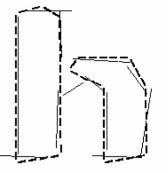
\includegraphics[scale=1]{broken-h.jpg}  
    \caption{Контур <<поломанной>> h}
    \label{fig:domain:recognition:tesseract:hcountor}
\end{figure}

Далее контуры отдаются классификатору, который строит набор из символов которым может быть наш распознаваемый и ищет наиболее похожий. Tesseract использует машинное обучение.

\subsubsection{}
OpenCv

OpenCv~\cite{open_cv_en} - библиотека алгоритмов компьютерного зрения, обработки изображений и численных алгоритмов общего назначения с открытым кодом. Библиотека поддерживает операционные системы Windows, Linux, Mac OS, iOS and Android, разрабатывается с упором для работы в режиме реального времени, имеет большое сообщество пользователей и хорошую поддержку от Intel. Очень хорошо сделанно взаимодействие с аппаратной частью компьютера. Не имеется достойных аналогов.

\subsection{Сборка и установка}
\label{sub:creation:build_and_install}

Для сборки програмного понадобится командная строка windows не ниже 7 версии

Для управления исходным кодом проекта используется система контроля версий Git \cite{git}. Прежде всего для компиляции требуется получить последнюю версию исходного кода программного средства. Перед получением исходного кода следует обратить внимание на значок результаты работы Continuous integration сервера, который можно найти на Readme странице с веб интерфейса git репозитории, он должен быть зеленого цвета это означает что последняя сборка была успешной, пример значка после успешной сборки можно увидеть на рисунке \ref{fig:domain:recognition:installation:success_build}.
\begin{figure}[ht] 
    \centering
    
\includegraphics[scale=1]{success_build.png}  
    \caption{Значок успешной сборки}
    \label{fig:domain:recognition:installation:success_build}
\end{figure}

Используя команду <<git clone>> нужно получить получить последнюю версию исходного кода програмного средства. Далее требуется получить библиотеки используемые в программном средстве. Все библиотеки загружаются через менеджер пакетов NuGet \cite{nuget}. Для получения пакетов следует воспользоваться командой nuget restore в директории с solution файлом. После загрузки библиотек можно приступать к сборке програмного средства. Для сборки понадобится MSBuild не ниже 14.0. Для начала сборки проекта следует воспользоваться командой: msbuild "src/vrpr.sln"  /property:Configuration= Release, артифакты сборки следует искать в директории <<src/vrpr.WebUi/bin/ Release>>. Для запуска сервера следует запустить <<vrpr.exe>> с правами администратора.